\documentclass[aspectratio=169]{beamer}

% Language setup
\usepackage[magyar]{babel} % Babel for Hungarian
\usepackage[T1]{fontenc} % Output character encoding
\usepackage[utf8]{inputenc} % Input character encoding
\selectlanguage{magyar}

% Beamer styling setup
\usetheme{Boadilla}
\usecolortheme{default}
%\setbeamercolor{titlelike}{parent=structure,bg=gray!15}
\setbeamertemplate{navigation symbols}{}
\setbeamertemplate{caption}[numbered]
%

% Spacing setup
\setlength{\parindent}{0pt} % No paragraph indenting
\setlength{\parskip}{5pt} % Set spacing between paragraphs
\frenchspacing
\newcommand{\mkspace}{\vspace{19pt}}
\newcommand{\rmspace}{\vspace{-19pt}}
\newcommand{\emptyline}{\vspace{\baselineskip}}
%

% Dependency setup
\usepackage{tikz}
\usetikzlibrary{decorations.markings}
\usetikzlibrary{calc}
%

% Style setup
\usepackage{caption}
\usepackage{subcaption}
\captionsetup{format=plain, font=footnotesize, labelformat=empty}
\usepackage{colortbl}
%

% Notation setup
\usepackage{physics} % Braket notation

% Add qi.svg logo
\usepackage{svg}
\usepackage[absolute,overlay]{textpos}

% Newline in cell
\usepackage{makecell}

\author[Nemkin Viktória]{Nemkin Viktória}
\institute[]{
\begin{small}dr. Friedl Katalin\end{small}\\
\begin{footnotesize}Számítástudományi és Információelméleti Tanszék\end{footnotesize}
}
\title{Memóriafelhasználás optimalizálása}
\subtitle{kvantumalgoritmusok szimulációja során}
\date{}

\begin{document}

\begin{frame}
\titlepage

\begin{textblock*}{150pt}(280pt,200pt) % {block width} (coords)
\includesvg[inkscape=overwrite,width=150pt]{./figures/qi.svg}
\end{textblock*}
\end{frame}


\begin{frame}{Motiváció: Protein folding kvantuszámítógépen}
\begin{columns}
\begin{column}{0.45\textwidth}
\begin{itemize}
    \item \textbf{Protein}:
    \begin{itemize}
        \item Aminosavakból alkotott lánc.
        \begin{itemize}
          \item \color{red} Piros = Hidrofób (''vízkerülő'').
          \item \color{blue} Kék = Poláris (''vízszerető'').
        \end{itemize}
        \item 3D kockarácson elhelyezve.
    \end{itemize}
    \item \textbf{Kódolás}:
    \begin{itemize}
        \item Origóból indul.
        \item Lépésenként $6$ irány $=$ $6$ ''qubit''.
    \end{itemize}
    \item \textbf{Orákulum}: 
    \begin{itemize}
        \item Energiaviszonyok lepontozása.
    \end{itemize}
    \item \textbf{Grover keresés}:
    \begin{itemize}
        \item Energiaminimum megtalálása.
        \item ''Kvantum párhuzamosság''-ot kihasználva.
    \end{itemize}
\end{itemize}
\end{column}
\begin{column}{0.55\textwidth}
\begin{figure}[H]
\center
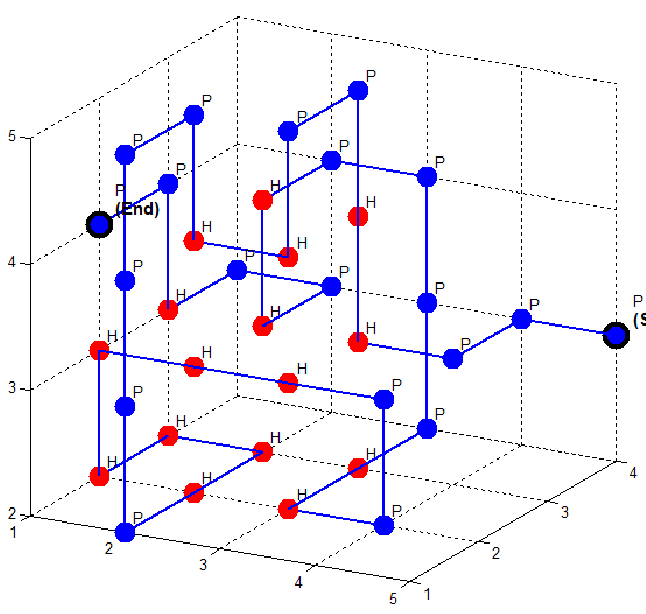
\includegraphics[width=0.8\textwidth]{./figures/Protein-folds-with-length-36-amino-acids-18-contacts.png}
\caption{Egy ''összehajtogatott'' protein.}
\end{figure}
\end{column}
\end{columns}

\end{frame}

\begin{frame}[t]{Probléma: Memóriahasználat}
\vspace{2mm}
\begin{tabular}{r|r|r|r}
Lánc & Qubitek & Regiszter & Operátor \\
\hline
\rule{0pt}{1.05\normalbaselineskip} $n$ & $6(n-1)$ & $2^{6(n-1)} \cdot{} 16 B$ & ${2^{12(n-1)}} \cdot{} 16 B$  \pause{} \\
\hline
2 & 6 &  1 KB &  64 KB \\
3 & 12 &  64 KB &  256 MB \\
4 & 18 &  4 MB & \color{red} 1 TB \\
5 & 24 &  256 MB & \color{red} 4 PB \\
6 & 30 &  16 GB & \color{red} 16384 PB \\
7 & 36 & \color{red} 1 TB & \color{red} 67108864 PB
\end{tabular}
\pause
\vspace{2mm}
\begin{itemize}
    \item Optimalizációk (regiszer és operátor esetében is):
    \begin{itemize}
        \item Ritka mátrixos tárolás.
        \begin{itemize}
          \item IBM Qiskit, Google Cirq, stb.
          \item Kevés, esetleges.
        \end{itemize}
        \item Döntési fa alapú adatszerkezet.
        \begin{itemize}
            \item Néhány éves cikkek.
        \end{itemize}
    \end{itemize}
\end{itemize}

\end{frame}

\definecolor{applegreen}{rgb}{0.55, 0.71, 0.0}

\begin{frame}[t]{Megoldás: ''On-the-fly'' és ''Függvény-alapú'' operátorok}
\vspace{2mm}
\begin{tabular}{r|r|r|r|r|r}
Lánc & Qubitek & Regiszter & Operátor &  \cellcolor{applegreen!30} ''On-the-fly'' &  \cellcolor{applegreen!30} ''Függvény-alapú'' \\
\hline
\rule{0pt}{1.05\normalbaselineskip} $n$ & $6(n-1)$ & $2^{6(n-1)} \cdot{} 16 B$ & ${2^{12(n-1)}} \cdot{} 16 B$ &  = Regiszter. &   Nem kell tárolni. \\
\hline
2 & 6 &  1 KB &  64 KB &  1 KB & 0 B \\
3 & 12 &  64 KB &  256 MB &  64 KB & 0 B \\
4 & 18 &  4 MB & \color{red} 1 TB &  4 MB & 0 B  \\
5 & 24 &  256 MB & \color{red} 4 PB &  256 MB & 0 B \\
6 & 30 &  16 GB & \color{red} 16384 PB &  16 GB & 0 B\\
7 & 36 & \color{red} 1 TB & \color{red} 67108864 PB & \color{red} 1 TB & 0 B
\end{tabular}
\pause
\vspace{2mm}
\begin{itemize}
    \item Qiskit, stb. nyílt forráskódúak...
    \item ...de szerves része a kódnak az operátor tárolása
    \item $\rightarrow$ saját szimulátor implementáció.
\end{itemize}

\end{frame}


\begin{frame}{Kvantumregiszterek állapotának tárolása}

\begin{itemize}
    \item Minden bitsorozathoz egy komplex valószínűségi amplítúdó.
    \item Szuperpozíció és összefonódás $\rightarrow$ több regiszterre ezek Descartes-szorzatát kell tárolni.
\end{itemize}

\begin{figure}[H]
    \centering
    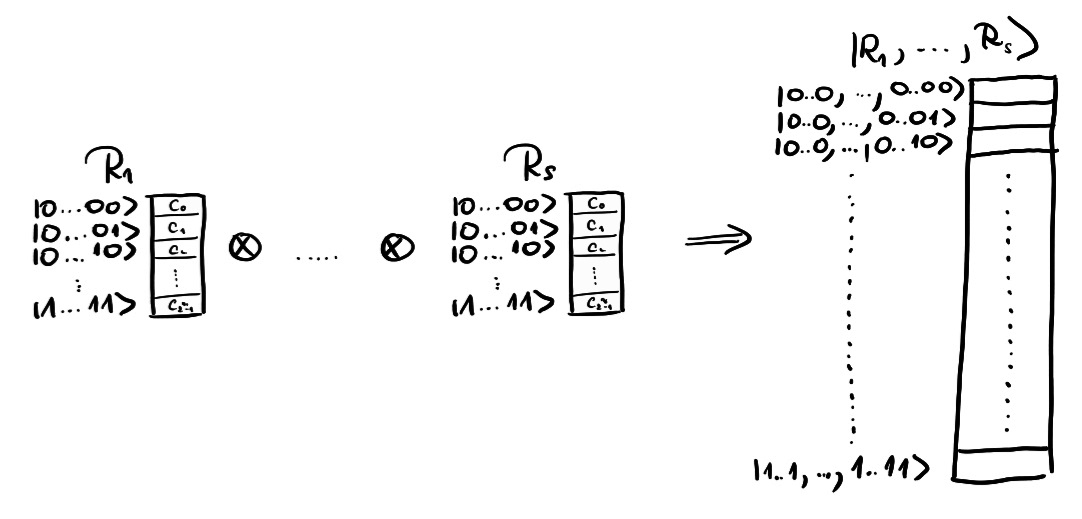
\includegraphics[width=0.7\textwidth]{figures/osszefonodas.jpg}
\end{figure}

\end{frame}

\begin{frame}{Operátor végrehajtás általánosan}

Az összes regiszterre: hagyományos mátrixszorzás.

\vspace{-0.4cm}
\begin{figure}[H]
    \centering
    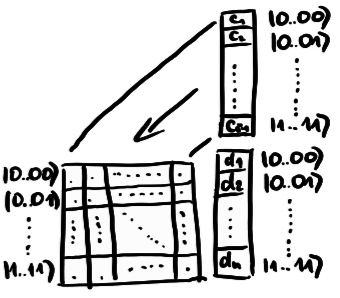
\includegraphics[width=0.3\textwidth]{figures/hagyomanyos_matrixszorzas.png}
\end{figure}

A rendszerben lévő regiszterek egy részhalmazára?

\begin{figure}[H]
    \centering
    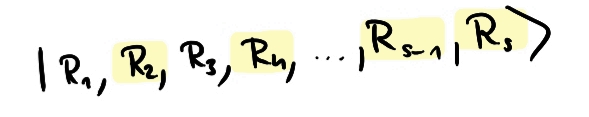
\includegraphics[width=0.4\textwidth]{figures/celregiszterek.png}
\end{figure}

\end{frame}


\begin{frame}{Mappelés}

\begin{figure}[H]
    \centering
    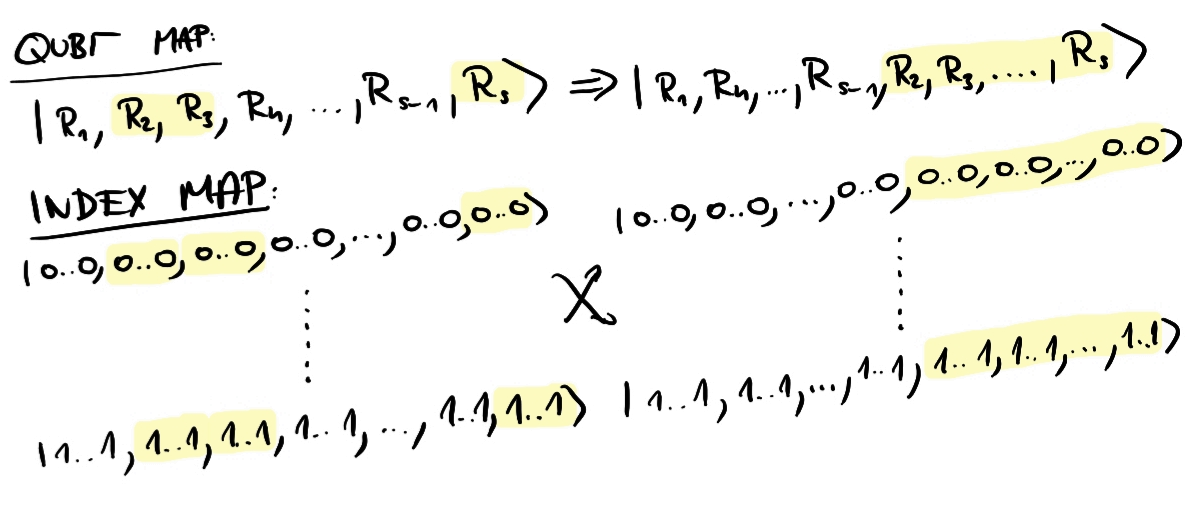
\includegraphics[width=\textwidth]{figures/mappeles.png}
\end{figure}

\end{frame}


\begin{frame}{Végrehajtás}

\begin{figure}[H]
    \centering
    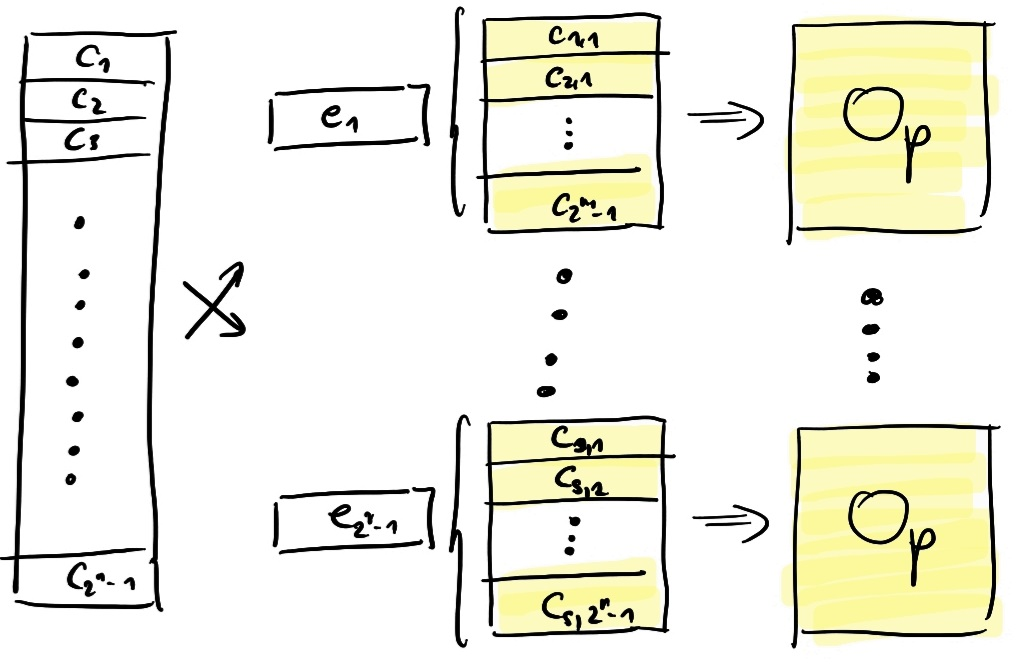
\includegraphics[width=0.7\textwidth]{figures/vegrehajtas.jpg}
\end{figure}

\end{frame}

\begin{frame}{Összegzés}

\begin{itemize}
    \item Qubit map
    \item Index map
    \item Group-by
    \item Csoportonként applyoljuk az operátort
    \begin{itemize}
        \item Nincs szükség egységmátrixszal tenzorszorozni.
        \item \#parallel-for pragmával ez párhuzamosítható.
    \end{itemize}
    \item Index map invertálása
\end{itemize}

\end{frame}

\begin{frame}{Operátorok}

\begin{itemize}
    \item Visitor minta / inverzió:
    \begin{itemize}
        \item Operátornak odaadom a regisztert, végrehajtja magát rajta.
        \item Belső működés eltakarva.
    \end{itemize}
    \item "On-the-fly" operátorok:
    \begin{itemize}
        \item Egy-egy regiszterrel egyező méretű sort generálok belőlük.
        \item Hadamard, Grover.
    \end{itemize}
    \item "Függvény-alapú" operátorok:
    \begin{itemize}
        \item $u: \ket{0\dots{}0,\text{in}} \rightarrow \ket{\text{out},\text{in}}$
        \item Sum: $\sum: \ket{0\dots{}0,\text{in}} \rightarrow \ket{\text{count}(\text{in}),\text{in}}$
        \item MC-NOT: $\text{mcnot}: \ket{0,\text{in}} \rightarrow \ket{\text{any}(\text{in}),\text{in}}$
    \end{itemize}
\end{itemize}


\end{frame}

\begin{frame}{Összegzés}

\begin{itemize}
\item Eredmények:
\begin{itemize}
    \item Ritka mátrixosan tárolt regiszerek.
    \item Regiszerkezelés tetszőleges célregiszerekkel.
    \item ''On-the-fly'' operátorok: Hadamard, Grover.
    \item ''Függvény-alapú'' operátorok: Sum, Multi-Controlled NOT.
    \item Könnyű bővíthetőség új operátorral.
\end{itemize}
\item Jövőbeli terv:
\begin{itemize}
    \item Protein folding algoritmus implementálása.
    \item Döntési fa alapú tárolás kipróbálása.
\end{itemize}
\end{itemize}

\end{frame}

\end{document}